\documentclass{article}
\usepackage{hyperref}
\usepackage[table,xcdraw]{xcolor}
\usepackage{xcolor}
\usepackage{graphicx}
\begin{document}
\title{Rapport de projet Picross}
\author{CONNES Victor, PRYSIAZHNIUK Anastasiia, saississez vos noms}
\maketitle
\tableofcontents 
\newpage
\section{Description du probl\`eme}

Le Picross est un casse-t\^ete qui consiste \`a retrouver une figure depuis les indices. La figure \`a d’ecouvrir est une grille dans laquelle chaque case est de couleur noire ou blanche. Pour chacune des lignes et colonnes on dispose d'un indice qui est une s\'equence de nombres repr\'esentant les longueurs des blocs de cases noires contigues de la ligne/colonne. Les blocs de cases noires sont s\'epar\'ees par au moins une case blanche.

\begin{table}[h]
\centering
\begin{tabular}{ccccccc}
\textbf{}  & \textbf{}                       & \textbf{3}                     & \textbf{4}                     & \textbf{4}                     & \textbf{4}                     & \textbf{3}                     \\ \cline{3-7} 
\textbf{2} & \multicolumn{1}{c|}{\textbf{2}} & \multicolumn{1}{c|}{\textbf{}} & \multicolumn{1}{c|}{\textbf{}} & \multicolumn{1}{c|}{\textbf{}} & \multicolumn{1}{c|}{\textbf{}} & \multicolumn{1}{c|}{\textbf{}} \\ \cline{3-7} 
\textbf{}  & \multicolumn{1}{c|}{\textbf{5}} & \multicolumn{1}{c|}{\textbf{}} & \multicolumn{1}{c|}{\textbf{}} & \multicolumn{1}{c|}{\textbf{}} & \multicolumn{1}{c|}{\textbf{}} & \multicolumn{1}{c|}{\textbf{}} \\ \cline{3-7} 
\textbf{}  & \multicolumn{1}{c|}{\textbf{5}} & \multicolumn{1}{c|}{\textbf{}} & \multicolumn{1}{c|}{\textbf{}} & \multicolumn{1}{c|}{\textbf{}} & \multicolumn{1}{c|}{\textbf{}} & \multicolumn{1}{c|}{\textbf{}} \\ \cline{3-7} 
\textbf{}  & \multicolumn{1}{c|}{\textbf{3}} & \multicolumn{1}{c|}{\textbf{}} & \multicolumn{1}{c|}{\textbf{}} & \multicolumn{1}{c|}{\textbf{}} & \multicolumn{1}{c|}{\textbf{}} & \multicolumn{1}{c|}{\textbf{}} \\ \cline{3-7} 
\textbf{}  & \multicolumn{1}{c|}{\textbf{1}} & \multicolumn{1}{c|}{\textbf{}} & \multicolumn{1}{c|}{\textbf{}} & \multicolumn{1}{c|}{\textbf{}} & \multicolumn{1}{c|}{\textbf{}} & \multicolumn{1}{c|}{\textbf{}} \\ \cline{3-7} 
\end{tabular}
\end{table}

\begin{table}[h]
\centering
\begin{tabular}{ccccccc}
\textbf{}  & \textbf{}                       & \textbf{3}                                                                    & \textbf{4}                                                                    & \textbf{4}                                                                    & \textbf{4}                                                                    & \textbf{3}                                                                    \\ \cline{3-7} 
\textbf{2} & \multicolumn{1}{c|}{\textbf{2}} & \multicolumn{1}{c|}{\cellcolor[HTML]{000000}{\color[HTML]{000000} \textbf{}}} & \multicolumn{1}{c|}{\cellcolor[HTML]{000000}\textbf{}}                        & \multicolumn{1}{c|}{\textbf{}}                                                & \multicolumn{1}{c|}{\cellcolor[HTML]{000000}\textbf{}}                        & \multicolumn{1}{c|}{\cellcolor[HTML]{000000}\textbf{}}                        \\ \cline{3-7} 
\textbf{}  & \multicolumn{1}{c|}{\textbf{5}} & \multicolumn{1}{c|}{\cellcolor[HTML]{000000}\textbf{}}                        & \multicolumn{1}{c|}{\cellcolor[HTML]{000000}\textbf{}}                        & \multicolumn{1}{c|}{\cellcolor[HTML]{000000}\textbf{}}                        & \multicolumn{1}{c|}{\cellcolor[HTML]{000000}\textbf{}}                        & \multicolumn{1}{c|}{\cellcolor[HTML]{000000}\textbf{}}                        \\ \cline{3-7} 
\textbf{}  & \multicolumn{1}{c|}{\textbf{5}} & \multicolumn{1}{c|}{\cellcolor[HTML]{000000}{\color[HTML]{000000} \textbf{}}} & \multicolumn{1}{c|}{\cellcolor[HTML]{000000}{\color[HTML]{000000} \textbf{}}} & \multicolumn{1}{c|}{\cellcolor[HTML]{000000}{\color[HTML]{000000} \textbf{}}} & \multicolumn{1}{c|}{\cellcolor[HTML]{000000}{\color[HTML]{000000} \textbf{}}} & \multicolumn{1}{c|}{\cellcolor[HTML]{000000}{\color[HTML]{000000} \textbf{}}} \\ \cline{3-7} 
\textbf{}  & \multicolumn{1}{c|}{\textbf{3}} & \multicolumn{1}{c|}{\textbf{}}                                                & \multicolumn{1}{c|}{\cellcolor[HTML]{000000}\textbf{}}                        & \multicolumn{1}{c|}{\cellcolor[HTML]{000000}\textbf{}}                        & \multicolumn{1}{c|}{\cellcolor[HTML]{000000}\textbf{}}                        & \multicolumn{1}{c|}{\textbf{}}                                                \\ \cline{3-7} 
\textbf{}  & \multicolumn{1}{c|}{\textbf{1}} & \multicolumn{1}{c|}{\textbf{}}                                                & \multicolumn{1}{c|}{\textbf{}}                                                & \multicolumn{1}{c|}{\cellcolor[HTML]{000000}\textbf{}}                        & \multicolumn{1}{c|}{\textbf{}}                                                & \multicolumn{1}{c|}{\textbf{}}   
                                             \\ \cline{3-7} 
\end{tabular}
\caption{Un exemple de Picross et sa solution.}
\end{table}

Certaines grilles peuvent ne pas avoir de solution ou en avoir plusieurs.
\begin{table}[h]
\centering
\begin{tabular}{
>{\columncolor[HTML]{FFFFFF}}c 
>{\columncolor[HTML]{FFFFFF}}c 
>{\columncolor[HTML]{FFFFFF}}c 
>{\columncolor[HTML]{FFFFFF}}c 
>{\columncolor[HTML]{FFFFFF}}c }
\textbf{}                                               & \textbf{2}                                                                    & \textbf{2}                                                                    & \textbf{2}                                                                    & \textbf{2}                                                                    \\ \cline{2-5} 
\multicolumn{1}{r|}{\cellcolor[HTML]{FFFFFF}\textbf{2}} & \multicolumn{1}{c|}{\cellcolor[HTML]{FFFFFF}{\color[HTML]{000000} \textbf{}}} & \multicolumn{1}{c|}{\cellcolor[HTML]{FFFFFF}\textbf{}}                        & \multicolumn{1}{c|}{\cellcolor[HTML]{FFFFFF}\textbf{}}                        & \multicolumn{1}{c|}{\cellcolor[HTML]{FFFFFF}\textbf{}}                        \\ \cline{2-5} 
\multicolumn{1}{c|}{\cellcolor[HTML]{FFFFFF}\textbf{2}} & \multicolumn{1}{c|}{\cellcolor[HTML]{FFFFFF}\textbf{}}                        & \multicolumn{1}{c|}{\cellcolor[HTML]{FFFFFF}\textbf{}}                        & \multicolumn{1}{c|}{\cellcolor[HTML]{FFFFFF}\textbf{}}                        & \multicolumn{1}{c|}{\cellcolor[HTML]{FFFFFF}\textbf{}}                        \\ \cline{2-5} 
\multicolumn{1}{c|}{\cellcolor[HTML]{FFFFFF}\textbf{2}} & \multicolumn{1}{c|}{\cellcolor[HTML]{FFFFFF}{\color[HTML]{000000} \textbf{}}} & \multicolumn{1}{c|}{\cellcolor[HTML]{FFFFFF}{\color[HTML]{000000} \textbf{}}} & \multicolumn{1}{c|}{\cellcolor[HTML]{FFFFFF}{\color[HTML]{000000} \textbf{}}} & \multicolumn{1}{c|}{\cellcolor[HTML]{FFFFFF}{\color[HTML]{000000} \textbf{}}} \\ \cline{2-5} 
\multicolumn{1}{c|}{\cellcolor[HTML]{FFFFFF}\textbf{2}} & \multicolumn{1}{c|}{\cellcolor[HTML]{FFFFFF}\textbf{}}                        & \multicolumn{1}{c|}{\cellcolor[HTML]{FFFFFF}\textbf{}}                        & \multicolumn{1}{c|}{\cellcolor[HTML]{FFFFFF}\textbf{}}                        & \multicolumn{1}{c|}{\cellcolor[HTML]{FFFFFF}\textbf{}}                        \\ \cline{2-5} 
\end{tabular}
\end{table}

\begin{table}[h]
\centering
\begin{tabular}{
>{\columncolor[HTML]{FFFFFF}}c 
>{\columncolor[HTML]{FFFFFF}}c 
>{\columncolor[HTML]{FFFFFF}}c 
>{\columncolor[HTML]{FFFFFF}}c 
>{\columncolor[HTML]{FFFFFF}}c }
\textbf{}                                               & \textbf{2}                                                                    & \textbf{2}                                                                    & \textbf{2}                                                                    & \textbf{2}                                                                    \\ \cline{2-5} 
\multicolumn{1}{r|}{\cellcolor[HTML]{FFFFFF}\textbf{2}} & \multicolumn{1}{c|}{\cellcolor[HTML]{000000}{\color[HTML]{000000} \textbf{}}} & \multicolumn{1}{c|}{\cellcolor[HTML]{000000}\textbf{}}                        & \multicolumn{1}{c|}{\cellcolor[HTML]{FFFFFF}\textbf{}}                        & \multicolumn{1}{c|}{\cellcolor[HTML]{FFFFFF}\textbf{}}                        \\ \cline{2-5} 
\multicolumn{1}{c|}{\cellcolor[HTML]{FFFFFF}\textbf{2}} & \multicolumn{1}{c|}{\cellcolor[HTML]{000000}\textbf{}}                        & \multicolumn{1}{c|}{\cellcolor[HTML]{000000}\textbf{}}                        & \multicolumn{1}{c|}{\cellcolor[HTML]{FFFFFF}\textbf{}}                        & \multicolumn{1}{c|}{\cellcolor[HTML]{FFFFFF}\textbf{}}                        \\ \cline{2-5} 
\multicolumn{1}{c|}{\cellcolor[HTML]{FFFFFF}\textbf{2}} & \multicolumn{1}{c|}{\cellcolor[HTML]{FFFFFF}{\color[HTML]{000000} \textbf{}}} & \multicolumn{1}{c|}{\cellcolor[HTML]{FFFFFF}{\color[HTML]{000000} \textbf{}}} & \multicolumn{1}{c|}{\cellcolor[HTML]{000000}{\color[HTML]{000000} \textbf{}}} & \multicolumn{1}{c|}{\cellcolor[HTML]{000000}{\color[HTML]{000000} \textbf{}}} \\ \cline{2-5} 
\multicolumn{1}{c|}{\cellcolor[HTML]{FFFFFF}\textbf{2}} & \multicolumn{1}{c|}{\cellcolor[HTML]{FFFFFF}\textbf{}}                        & \multicolumn{1}{c|}{\cellcolor[HTML]{FFFFFF}\textbf{}}                        & \multicolumn{1}{c|}{\cellcolor[HTML]{000000}\textbf{}}                        & \multicolumn{1}{c|}{\cellcolor[HTML]{000000}\textbf{}}                        \\ \cline{2-5} 
\end{tabular}
\end{table}
\newpage

\begin{table}[h]
\centering
\begin{tabular}{
>{\columncolor[HTML]{FFFFFF}}c 
>{\columncolor[HTML]{FFFFFF}}c 
>{\columncolor[HTML]{FFFFFF}}c 
>{\columncolor[HTML]{FFFFFF}}c 
>{\columncolor[HTML]{FFFFFF}}c }
\textbf{}                                               & \textbf{2}                                                                    & \textbf{2}                                                                    & \textbf{2}                                                                    & \textbf{2}                                                                    \\ \cline{2-5} 
\multicolumn{1}{r|}{\cellcolor[HTML]{FFFFFF}\textbf{2}} & \multicolumn{1}{c|}{\cellcolor[HTML]{FFFFFF}{\color[HTML]{000000} \textbf{}}} & \multicolumn{1}{c|}{\cellcolor[HTML]{FFFFFF}\textbf{}}                        & \multicolumn{1}{c|}{\cellcolor[HTML]{000000}\textbf{}}                        & \multicolumn{1}{c|}{\cellcolor[HTML]{000000}\textbf{}}                        \\ \cline{2-5} 
\multicolumn{1}{c|}{\cellcolor[HTML]{FFFFFF}\textbf{2}} & \multicolumn{1}{c|}{\cellcolor[HTML]{FFFFFF}\textbf{}}                        & \multicolumn{1}{c|}{\cellcolor[HTML]{FFFFFF}\textbf{}}                        & \multicolumn{1}{c|}{\cellcolor[HTML]{000000}\textbf{}}                        & \multicolumn{1}{c|}{\cellcolor[HTML]{000000}\textbf{}}                        \\ \cline{2-5} 
\multicolumn{1}{c|}{\cellcolor[HTML]{FFFFFF}\textbf{2}} & \multicolumn{1}{c|}{\cellcolor[HTML]{000000}{\color[HTML]{000000} \textbf{}}} & \multicolumn{1}{c|}{\cellcolor[HTML]{000000}{\color[HTML]{000000} \textbf{}}} & \multicolumn{1}{c|}{\cellcolor[HTML]{FFFFFF}{\color[HTML]{000000} \textbf{}}} & \multicolumn{1}{c|}{\cellcolor[HTML]{FFFFFF}{\color[HTML]{000000} \textbf{}}} \\ \cline{2-5} 
\multicolumn{1}{c|}{\cellcolor[HTML]{FFFFFF}\textbf{2}} & \multicolumn{1}{c|}{\cellcolor[HTML]{000000}\textbf{}}                        & \multicolumn{1}{c|}{\cellcolor[HTML]{000000}\textbf{}}                        & \multicolumn{1}{c|}{\cellcolor[HTML]{FFFFFF}\textbf{}}                        & \multicolumn{1}{c|}{\cellcolor[HTML]{FFFFFF}\textbf{}}                        \\ \cline{2-5} 
\end{tabular}
\caption{Un exemple de Picross qui a deux solutions.}
\end{table}

\begin{table}[h]
\centering
\begin{tabular}{lccccc}
                   & \multicolumn{1}{l}{}                                    & \multicolumn{1}{l}{\textbf{1}}                                                & \multicolumn{1}{l}{\textbf{}}                                                 & \multicolumn{1}{l}{\textbf{}}                                                 & \multicolumn{1}{l}{\textbf{1}}                                                \\
                   & \cellcolor[HTML]{FFFFFF}\textbf{}                       & \cellcolor[HTML]{FFFFFF}\textbf{1}                                            & \cellcolor[HTML]{FFFFFF}\textbf{1}                                            & \cellcolor[HTML]{FFFFFF}\textbf{1}                                            & \cellcolor[HTML]{FFFFFF}\textbf{1}                                            \\ \cline{3-6} 
\textbf{1}         & \multicolumn{1}{c|}{\cellcolor[HTML]{FFFFFF}\textbf{1}} & \multicolumn{1}{c|}{\cellcolor[HTML]{FFFFFF}\textbf{}}                        & \multicolumn{1}{c|}{\cellcolor[HTML]{FFFFFF}\textbf{}}                        & \multicolumn{1}{c|}{\cellcolor[HTML]{FFFFFF}\textbf{}}                        & \multicolumn{1}{c|}{\cellcolor[HTML]{FFFFFF}{\color[HTML]{000000} \textbf{}}} \\ \cline{3-6} 
\rowcolor[HTML]{FFFFFF} 
\textit{\textbf{}} & \multicolumn{1}{c|}{\cellcolor[HTML]{FFFFFF}\textbf{3}} & \multicolumn{1}{c|}{\cellcolor[HTML]{FFFFFF}{\color[HTML]{000000} \textbf{}}} & \multicolumn{1}{c|}{\cellcolor[HTML]{FFFFFF}{\color[HTML]{000000} \textbf{}}} & \multicolumn{1}{c|}{\cellcolor[HTML]{FFFFFF}{\color[HTML]{000000} \textbf{}}} & \multicolumn{1}{c|}{\cellcolor[HTML]{FFFFFF}{\color[HTML]{000000} \textbf{}}} \\ \cline{3-6} 
\textbf{1}         & \multicolumn{1}{c|}{\cellcolor[HTML]{FFFFFF}\textbf{1}} & \multicolumn{1}{c|}{\cellcolor[HTML]{FFFFFF}\textbf{}}                        & \multicolumn{1}{c|}{\cellcolor[HTML]{FFFFFF}\textbf{}}                        & \multicolumn{1}{c|}{\cellcolor[HTML]{FFFFFF}\textbf{}}                        & \multicolumn{1}{c|}{\cellcolor[HTML]{FFFFFF}\textbf{}}                        \\ \cline{3-6} 
\end{tabular}
\end{table}


\begin{table}[h]
\centering
\begin{tabular}{lccccc}
                                           & \multicolumn{1}{l}{}                                             & \multicolumn{1}{l}{\textbf{1}}                                                & \multicolumn{1}{l}{\textbf{}}                                                 & \multicolumn{1}{l}{\textbf{}}                                                 & \multicolumn{1}{l}{\textbf{1}}                                                \\
                                           & \cellcolor[HTML]{FFFFFF}\textbf{}                                & \cellcolor[HTML]{FFFFFF}\textbf{1}                                            & \cellcolor[HTML]{FFFFFF}\textbf{1}                                            & \cellcolor[HTML]{FFFFFF}\textbf{1}                                            & \cellcolor[HTML]{FFFFFF}\textbf{1}                                            \\ \cline{3-6} 
\textbf{1}                                 & \multicolumn{1}{c|}{\cellcolor[HTML]{FFFFFF}\textbf{1}}          & \multicolumn{1}{c|}{\cellcolor[HTML]{000000}\textbf{}}                        & \multicolumn{1}{c|}{\cellcolor[HTML]{FFFFFF}\textbf{}}                        & \multicolumn{1}{c|}{\cellcolor[HTML]{FFFFFF}\textbf{}}                        & \multicolumn{1}{c|}{\cellcolor[HTML]{000000}{\color[HTML]{000000} \textbf{}}} \\ \cline{3-6} 
\cellcolor[HTML]{FFFFFF}\textit{\textbf{}} & \multicolumn{1}{c|}{\cellcolor[HTML]{FFFFFF}\textit{\textbf{3}}} & \multicolumn{1}{c|}{\cellcolor[HTML]{9B9B9B}{\color[HTML]{000000} \textbf{}}} & \multicolumn{1}{c|}{\cellcolor[HTML]{000000}{\color[HTML]{000000} \textbf{}}} & \multicolumn{1}{c|}{\cellcolor[HTML]{000000}{\color[HTML]{000000} \textbf{}}} & \multicolumn{1}{c|}{\cellcolor[HTML]{9B9B9B}{\color[HTML]{000000} \textbf{}}} \\ \cline{3-6} 
\textbf{1}                                 & \multicolumn{1}{c|}{\cellcolor[HTML]{FFFFFF}\textbf{1}}          & \multicolumn{1}{c|}{\cellcolor[HTML]{000000}\textbf{}}                        & \multicolumn{1}{c|}{\cellcolor[HTML]{FFFFFF}\textbf{}}                        & \multicolumn{1}{c|}{\cellcolor[HTML]{FFFFFF}\textbf{}}                        & \multicolumn{1}{c|}{\cellcolor[HTML]{000000}\textbf{}}                        \\ \cline{3-6} 
\end{tabular}
\caption{Un exemple de Picross qui n'a pas de solution.}
\end{table}
\newpage
La r\'esolution du Picross est un probl\`eme NP-complet( NP-Complet est un probl\`eme difficile \`a r\'esoudre, par exemple, le probl\`eme SAT). Pour le probl\`eme du Picross cela signifie qu\'il ne faut pas esp\'erer un algorithme qui r\'esout n\'importe quelle grille de Picross avec une complexit\'e polynomiale (en fonction de la taille de la grille) dans le pire des cas. En plus, la difficult\`e de r\'esolution varie selon la taille du grille.

Le but du projet s'agit d'implanter un solveur de Picross en C++ qui lit les donn\'ees d'un probl\`eme Picross, calcule puis affiche sa solution. On ne consid\`ere que des Picross qui ont une solution unique (contrainte donn\'ee dans le cahier des charges).





\section{Description de l'impl\'ementation}
\subsection{ Les besoins du programme :}

\subsubsection{Pour les indices de chaque ligne/colonne:}
\begin{itemize}
\item Imperatif \`a satisfaire:
\begin{itemize}

\item structure de taille dynamique (nombre variable d’indice par ligne)
\item parcours en $\theta$(n) (plusieurs m\'ethodes recourant \`a  un parcours total ou partiel de la structure)
\item relation d’ordre (le parcours ne sont r\'ealiser que dans l’ordre de l’indice le plus en haut vers celui le plus en bas respectivement gauche-droite pour les
lignes)
\end{itemize}
\item Choix : la liste simplement chain\'es, car elle correspond parfaitement au sp\'ecification et parait finalement tr\`es proche de la r\'ealit\'e
\end{itemize}
\subsubsection{Pour repr\'esenter la grille du picross :}
\begin{itemize}
\item Imperatif \`a satisfaire:
\begin{itemize}
\item structure de taille fixe
\item acc\`es en temps constant a chaque case
\item faciliter de copie de la structure ($\theta$(n))
\end{itemize}
\item Choix: La matrice car tr\`es proche de la r\'ealit\'e
\end{itemize}
\subsubsection{Pour l’ensemble des indices de lignes/colonnes :}
\begin{itemize}
\item Imperatif \`a satisfaire:
\begin{itemize}
\item acc\'eder en temps constant a chaque liste
\item garder un indicage coh\'erent avec la matrice
\end{itemize}
\item Choix :Un tableau
\end{itemize}
\subsubsection{Pour ligmodif /colmodif}
\begin{itemize}
\item Imperatif \`a satisfaire:
\begin{itemize}
\item ajout d’un \'el\'ement en temps constant
\item retrait d’un \'el\'ement en temps constant
\item taille dynamique
\end{itemize}
\item Choix :
Le choix naturel serait l’ensemble mais on choisit la liste simplement chain\'es car d\'ej\`a  impl\'ement\'es pour les indices de chaque ligne/colonne. Son
comportement est similaire dans le cas d'un ajout et d'un retrait en d\'ebut de liste .
\end{itemize}
\subsection{ Les classes}
L'ensemble de nos classes disposent d'une surcharge de l'operateur<< afin de faciliter l'affichage dans le terminal. De plus, il existe d'autres classes dans notre
programme qui permettent d'am\'eliorer l'affichage en utilisant une interface graphique. Nous ne distinguerons ici seulement les classes permettant la
resolution du picross.

\subsubsection{La classe Cell :}
Elle repr\'esente un indice logique
\begin{itemize}
\item Attributs :
\begin{itemize}
\item Val : qui repr\'esente la valeur de cette indice logique (cette valeur \'etant strictement enti\`ere positive et a priori non born\'e nous avons choisit de la repr\'esenter par un short int)
\item Suiv : qui est pointeur sur la cellule suivante de la liste
\end{itemize}
\end{itemize}
\subsubsection{La classe Liste :}
\begin{itemize}
\item Attributs :
\begin{itemize}
\item Longueur : qui repr\'esente la longueur de la liste. Cette attribut et incr\'ementer ou d\'ecr\'ementer automatiquement d\`es qu'il y a variations de la taille de la
liste.
\item Fini : Nous indique si la ligne/colonne a laquelle est rattach\'e la liste est enti\`erement rempli (bool\'een \`a  true) ou non (bool\'een \`a  false), cette attribut et
notamment tr\`es utile pour v\'erifier la condition d'arrêt de notre r\'esolution (cf. main)
\item Tête : Pointeur vers le premier \'el\'ement de la liste.
\end{itemize}
\item M\'ethode remarquable :
\begin{itemize}
\item Surcharge de l'op\'erateur() : Nous avons utiliser l'operateur() comme un operateur d'indexage d'une liste cela nous permet notamment de faciliter le
parcours d'une liste.
\end{itemize}
\end{itemize}
\subsubsection{La classe Tabliste :}
\begin{itemize}
\item Attributs :
\begin{itemize}
\item Tab : le tableau de liste
\item Taille : la taille du tableau
\end{itemize}
\item M\'ethode remarquable :
\begin{itemize}
\item Surcharge de l'op\'erateur[]: Nous permet d'utiliser comme si elle \'etait simplement un tableau.
\end{itemize}
\end{itemize}
\subsubsection{La classe Matrice :}
\begin{itemize}
\item Attributs:
\begin{itemize}
\item Tab : la matrice d'entier (-1 : blanc 0 : ind\'etermin\'e 1 : noir)
\item Nbl : Nombre de ligne
\item Nbc : Nombre de colonnes
\end{itemize}
\end{itemize}
\subsection{ La classe Picross :}
La classe picross est la classe dont les instances repr\'esente les picross c'est dans cette classe que sont impl\'ement\'e nos m\'ethodes de r\'esolution.
\subsection{Les algorithmes remarquables :}
\subsubsection{SLG :}
\paragraph{Sp\'ecification :}
 void SLG(int*, short int, Cell*, short int, bool\&);
\begin{itemize}
\item Param\`etre:
\begin{itemize}
\item Un tableau d'entier: (Donée/resultat) il repr\'esente une ligne/colonne de notre matrice, initialement il peut contenir des cellules \`a 1,-1,0
\item Un short int : repr\'esentant la taille du tableau
\item Une cellule de liste: il rep\'esente le prochain indice a placer dans le tableau, initialement la premi\`ere cellule associ\'e \`a la dites ligne/colonnes
\item Un short int : repr\'esentant l'indice dans le tableau auquel on souhaite placer le bloc, initialement 0
\item Un bool\'een passé par r\'ef\'erence : représentant si il est possible ou non de placer la fin de la liste d'indices indice courant compt\'e a partir de l'indice courant dans le tableau.
\end{itemize}
\item Retour de la fonction.
\end{itemize}
Le retour ce fait par linterm\'ediaire du tableau  et du bool\'een. Si le bool\'een est \`a false c'est que le couple (ligne/colonne,liste d'indice) n'a pas de solution.Dans le cas contraire, la solution la plus \`a gauche nous est don\'ée dans le tableau.

\paragraph{Complexit\'e c pire des cas : $\theta(n^2) <$c$\leq\theta(2^n)$\\ }
 Notons :
\begin{itemize}
\item i: l'indice dans notre tableau
\item n: la taille du dit tableau
\item T: le dit tableau
\item l: la taille de la liste d'indice (le nombre d'indices)
\item $m_i$: l'envergure d'un indice i
\end{itemize}
Dans le pire des cas de notre algorythme, on peut imaginer que chaque hypoth\'ese faites par notre algorythme soit fausse notre fonction: Pour cela,il nous faut imaginer une liste d'indice de petite taille (ici on choisira $\forall$i $\in$[0,l[ $m_i$=1) en effet,plus les indices sont grand moins il ont de position possible pour une m\^eme taille de tableau, et donc moins d'hypothèse.
\newline Enfin,on voit bien que la complexit\'e vas d\'ependre de taille de la liste ,en effet,chaque cellule appelle la fonction au moins une fois pour chaque maillons placer après dans liste.Au plus,pour un indice j de la liste SLG sera appeé $\sum_{i=l-j}^{l} (i)$ fois c'est à dire l-i fois $\forall$i $\in$[j,l[.
\newline En outre, on sait que le co\^ut de SLG sans les appels r\'ecursif reviens a n puisque dans tous les cas o\`u la liste n'est pas vide ont recopie le tableau.Sinon, si la liste est vide on parcours le tableau de l'indice i à n, ici, on considerera cette valeur cst=n, n\'eanmoins bien que ce cas soit defavorable il n'est pas r\'ealiste en effet, dans le cas d'une liste non-vide ( ce qui notre cas) alors cette valeur est necessairement inférieure et decroit tout au long des appels de SLG.
Soit une complexit\'e inf\'erieure \`a $2^n$.
\newline
Avec ce modèle défavorable on obtient l'equation de recursion suivante:
\begin{center}
 \fbox{SLG(i)= $\sum_{k=l-i}^{l} (SLG(k)*n)+cst$}
\end{center}
Ainsi en notant c la complexité dans ce pire des cas: $\theta(n^2) <$c$\leq\theta(2^n)$,en effet, pour chaque case on parcours au minimun un fois le tableau (la recopie) pour chaque cellule après ici cela fait d\'ej\`a $\theta(n^2)$ et on doit le faire pour chaque indice.
\paragraph{Complexit\'e meilleur des cas : $\theta$(n)\newline}
Dans le meilleur des cas la liste est vide on doit pacourir une fois le tableau pour pouvoir v\'erifi\'e .
\subsubsection{Backtrack :}
\paragraph{Sp\'ecification :}
 void backtrack(bool \&poss);
\begin{itemize}
\item Param\`etre:
\begin{itemize}
\item Un booléen signalant la possibilitée de placer une case dans un picross non fini
\end{itemize}
Dans le cas ou cela est possible, on "backtrack" une case
Dans le cas ou cela n'est pas possible, on revient à l'environnement de la dernière case backtrackée et on l'inverse
\item Retour de la fonction.
\end{itemize}
La fonction ne retourne rien, on travaille directement sur notre Matrice.\newline
Cela à pour conséquence une complexité élevée ($\theta$(n)) lors de la recopie de celle-ci.
\subsubsection{Fusion :}
\paragraph{Sp\'ecification :}Fusion(int* Merge,int* TG,int* TD,sint taille);
\begin{itemize}
\item Param\`etre:
\begin{itemize}
\item Un tableau d'entier Merge: (Resultat) il repr\'esente la ligne/colonne de la matrice,après la resolution de notre fonction, initialisé avec la ligne/colonne existante
\item Un tableau d'entier TG: (Donn\'ee) il repr\'esente la solution la plus à gauche qui résout notre ligne/colonne en fonction de sa liste d'indices et des information à notre disposition
\item Un tableau d'entier TD: (Donn\'ee) idem pour la solution la plus à droite
\item Un short int taille: représentant la taille du tableau
\end{itemize}
\item Retour de la fonction:
\end{itemize}
La fonction retourne par l'interm\'ediaire du tableau Merge notre ligne/colonne de depart avec en plus d'enventuelle case noire "sures".
\paragraph{Comlexit\'e : $\theta$(n)\newline}
Nous parcourons chaque case du tableau pour v\'erifier si nous avons des informations suplementaires. Remarque: on aurait pu gérer une liste des indices qui était encore ind\'etermin\'e pour chaque ligne/colonne ce qui aurait am\'eliorer notre complexit\'e moyenne. N\'eanmoins, nous avons juger cela peut indispensable au vue du caract\`ere negligeble de cette complexit\'e par rapport au autre fonctions du programme. 
\subsubsection{remplirCasesSureBl :}
\paragraph{Sp\'ecification :}remplirCasesSureBl(int* Merge, int* TG,int* TD, sint taille, Liste \&L);
\begin{itemize}
\item Param\`etre:
\begin{itemize}
\item Un tableau d'entier Merge: (Resultat) il repr\'esente la ligne/colonne de la matrice,après la resolution de notre fonction, initialisé avec le retour de fusion.
\item Un tableau d'entier TG: (Donn\'ee) il repr\'esente la solution la plus à gauche qui résout notre ligne/colonne en fonction de sa liste d'indices et des information à notre disposition
\item Un tableau d'entier TD: (Donn\'ee) idem pour la solution la plus à droite
\item Un short int taille: représentant la taille du tableau
\item Une liste d'indices L: La liste d'indices associ\'es a la ligne/colonne
\end{itemize}
\item Retour de la fonction:
\end{itemize}
La fonction retourne par l'interm\'ediaire du tableau Merge notre ligne/colonne de depart avec en plus d'enventuelle case blanche "sures" en se basant sur l'envergure des blocs.
\paragraph{Comlexit\'e : $\theta(n)$\newline}
On doit pour chaque indice de la liste inscrire son envergure dans un tableau intermediaire pour cela il nous faut parcourir SLG puis SLD mais pas en totalit\'e ,en effet, on parcours SLG jusqu'a trouver un indice i1 tel que TG[i1]=0.On continu notre parcours jusqu'a trouver un indice i2 tel que TG[i2]=0,c'est alors, qu'on parcours SLD \`a partir de i2-1 jusqu'a trouver un indice i3 tel que TG[i3]=0. On a alors l'envergure du premier bloc.Pour le deuxi\'eme on peut commencer notre parcours dans SLG \'a partir de i2 car il est forc\'ement \`a droite du premier.\newline On trouve alors un nouveau i1 puis un i2 puis un i3 et on recommence alors \'a partir du nouveau i2 et ainsi de suite.Au final, on aura parcouru entre n et 2n case du tableau.

\subsubsection{remplirCaseBlcoince :}
\paragraph{Sp\'ecification :}CaseBlcoince(int* Merge, sint taille, Liste \&L);
\begin{itemize}
\item Param\`etre:
\begin{itemize}
\item Un tableau d'entier Merge: (Resultat) il repr\'esente la ligne/colonne de la matrice.
\item Un short int taille: représentant la taille du tableau
\item Une liste d'indices L: La liste d'indices associ\'es a la ligne/colonne
\end{itemize}
\item Retour de la fonction:
\end{itemize}
La fonction retourne par l'interm\'ediaire du tableau Merge notre ligne/colonne de depart avec en plus d'\'eventuelle case blanche "sures" en se basant sur les tailles des blocs.
\paragraph{Comlexit\'e : $\theta(n)$\newline}
\section{Description de la m\'ethode de r\'esolution utilis\'ee}
Afin de r\'esoudre une grille de Picross donn\'ee, nous traitons ses lignes ind\'ependamment de ses colonnes. 
Le traitement des lignes et des colonnes se faisant de la m\^eme mani\`ere; nous n'\'evoquerons par la suite que le traitement des lignes.
\newline
Une premi\`ere m\'ethode de r\'esolution consisterait \`a g\'en\'erer toutes les solutions d'une ligne, partiellement remplie ou non; et de d\'eterminer les cases noires ou blanches communes \`a chacune des solutions.
\newline
Une telle m\'ethode permettrait de d\'eterminer un grand nombre de cases. En revanche, c'est une m\'ethode tr\`es co\^uteuse.
\newline
C'est pourquoi, au lieu de g\'en\'erer toutes les solutions, nous avons choisi d'en g\'en\'erer deux; la plus \`a gauche et la plus \`a droite. Cette m\'ethode ne permet pas de d\'eterminer autant de cases que la pr\'ec\'edente mais elle est nettement moins co\^uteuse.
\subsection{La m\'ethode SLG}
La m\'ethode SLG a pour but de g\'en\'erer une solution \`a une ligne contenant ou non des cases d\'ej\`a d\'etermin\'ees.
Elle cherchera \`a placer chacun des blocs de la liste d'indices \`a partir d'un indice i dans la ligne.
Une fois un bloc plac\'e, elle cherchera \`a placer le suivant. Si elle n'y parvient pas, elle recommence en i+1.
Afin d'expliciter son fonctionnement, son algorithme est d\'etaill\'ee ci-dessous.
\paragraph{Algorithme : SLG}(L: ligne; n: taille de la ligne; Lind: liste d'indices; i: entier; possible: booleen)
\begin{description}
\item[Debut]
\item[]
  \begin{itemize}
  \item[Si] Lind est vide alors 
    \begin{itemize}
    \item[Si] L ne contient pas de cases noires alors
      \begin{itemize}
      \item possible == vrai;
      \end{itemize}
    \item[Si] possible alors
      \begin{itemize}
      \item on blanchit toutes les cases de L;
      \end{itemize}
    \end{itemize}
  \item[Sinon]
    \begin{itemize}
    \item[Si] l'espace entre i et n est insuffisant pour placer le bloc ou qu'on ne peut pas placer de case blanche apr\`es le bloc ou que l'espace entre i \`a la taille du bloc contient une case blanche alors
      \begin{itemize}
      \item possible == faux;
      \item On rappelle SLG avec i = i+1;
      \end{itemize}
    \item[Si] possible alors 
      \begin{itemize}
    \item On place le bloc \`a partir de i;
    \item On rappelle SLG pour l'indice de bloc suivant avec i = i+valeur d'indice pr\'ec\'edent+1;
      \end{itemize}
    \end{itemize}
  \end{itemize}
\item[Fin algorithme]
\end{description}
\subsection{R\'esolution d'une ligne}
\subsubsection{Les m\'ethodes SLPG et SLPD}
Les m\'ethodes SLPG et SLPD g\'en\`erent respectivement pour une ligne, sa solution la plus \`a gauche et sa solution la plus \`a droite. Elles font toutes deux appel \`a SLG avec i=0 et possible = faux. 
\newline
Pour la solution droite, SLG est appel\'e sur une ligne et une liste d'indices pr\'ealablement invers\'ees.
\subsubsection{La m\'ethode Fusion}
A la suite des appels \`a SLPG et SLPD, nous aurons deux solutions possibles pour une ligne; or, pour parvenir \`a la r\'esolution de notre Picross, il nous faut d\'eterminer les cases n'ayant qu'une solution. 
\newline
Pour ce faire, on fait appel \`a Fusion qui ne gardera que les cases noires communes aux deux solutions.
Cette derni\`ere n\'ecessite que nos blocs de cases noires soient num\'erot\'ees (appel \`a la m\'ethode Numeroter).
\newline
En effet, le status de case noire s\^ure ne peut \^etre d\'efini que si une case noire commune aux deux solutions appartient \`a un m\^eme et une unique bloc.
\newline
L'exemple ci-dessous illustre l'importance de cette sp\'ecification.  
\newline
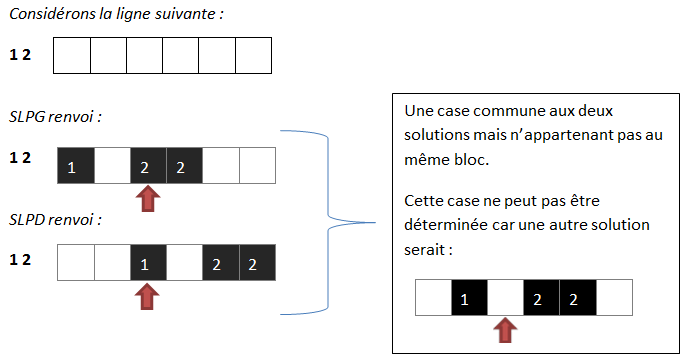
\includegraphics[height=6.5cm,width=12cm]{Exemple1}
\subsubsection{La m\'ethode remplirCasesSureBl}
Cette m\'ethode est appel\'ee apr\`es Fusion dans le but de placer les cases blanches s\^ures. Elle est en mesure de les d\'eterminer gr\^ace aux solutions SLPG-SLPD en calculant les envergures des blocs de cases noires. D\`es lors, les espaces situ\'es entre les intervalles trouv\'es sont des cases blanches s\^ures.
\paragraph{remplirCasesSureBl} commence par g\'en\'erer une ligne de cases blanche de la m\^eme taille que celles prises en param\'etre; \`a savoir, le r\'esultat de Fusion et les solutions SLPG-SLPD; puis ``noircit'' les cases correspantes \`a l'intervalle qu'occupe chacun des blocs dans l'une et l'autre des solutions SLPG-SLPD.
\newline
A la fin de ce proc\'ed\'e, elle copie les cases blanches restantes dans le r\'esultat de Fusion.
\subsubsection{Ajout de la ligne \`a la grille de Picross}
Une fois les cases s\^ures noires et blanches ajout\'ees \`a notre ligne, on v\'erifie par la m\'ethode isFini si elle compl\`ete ou non, afin de ne plus la traiter si tel est le cas.
\newline
Ensuite, on ajoute les indices des cases qui ont \'et\'e modifi\'ees \`a une liste appel\'ees colModif. Celle-ci permettra de traiter par la suite les colonnes o\`u une case \`a \'et\'e ajout\'ee.
\newline
Pour finir, on recopie notre ligne ainsi compl\'et\'ee dans la grille de Picross.
\end{document}
